\subsection*{Evaluation Lösungsprinzipien}\label{mk}
\addcontentsline{toc}{subsection}{Evaluation Lösungsprinzipien}


Aus der vorhergehenden Technologierecherche (siehe Anhang \nameref{techrecherche}) wird pro Teilbereich ein morphologischer Kasten erstellt. Dieser wird befüllt mit den Teilfunktionen und den recherchierten Technologien. Damit werden die Lösungsprinzipien evaluiert und verschiedene Varianten werden ausarbeitet. Nachfolgend sind alle morphologischen Kästen aufgezeigt.

\subsubsection*{Mechanik Morphologischer Kasten}
\addcontentsline{toc}{subsubsection}{Mechanik Morphologischer Kasten}

Die Lösungsansätze der Mechanik wurden nach folgenden Kriterien erstellt und in Tabelle \ref{table:mk-mechanik} in einem morphologischen Kasten dargestellt.

\begin{itemize}
    \item Variante Gelb: Effizient
    \item Variante Rot: Präzise
    \item Variante Grün: Robust
\end{itemize}

\begin{table}[H]
\centering
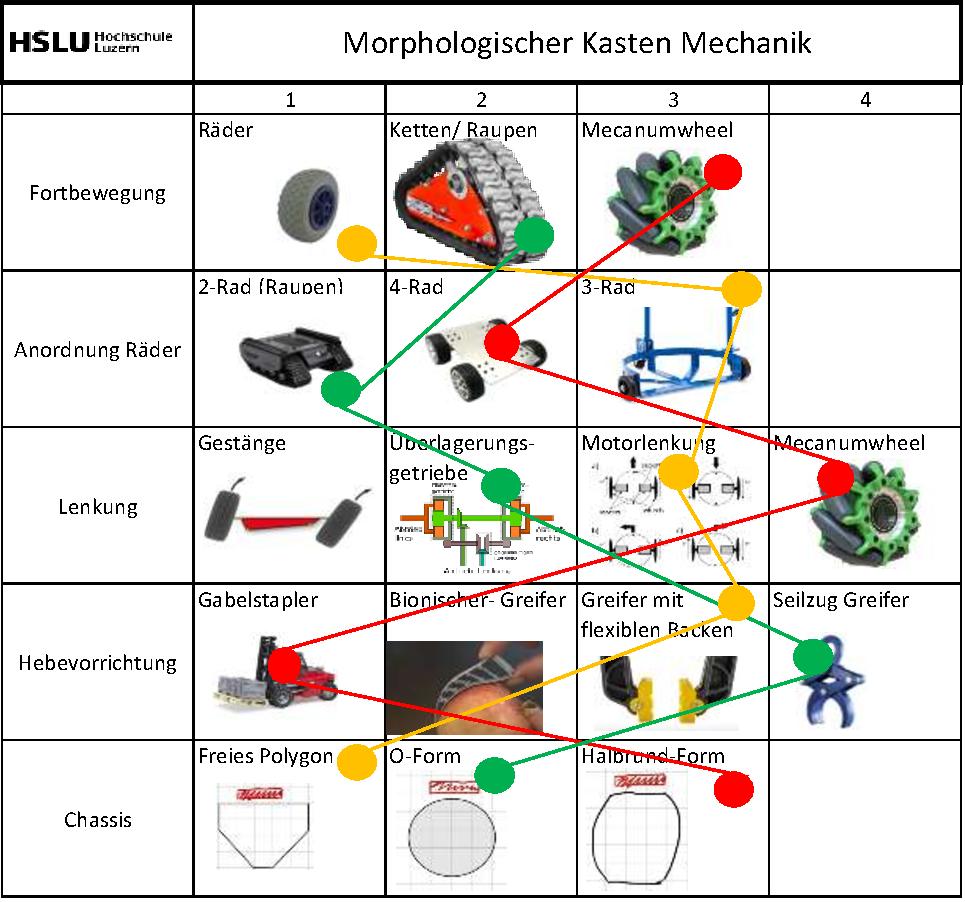
\includegraphics[width=0.7\textwidth]{assets/MK_Maschinentechnik.pdf}
\caption{Morphologischer Kasten: Mechanik}
\label{table:mk-mechanik}
\end{table}


\subsubsection*{Steuerung Morphologischer Kasten}
\addcontentsline{toc}{subsubsection}{Steuerung Morphologischer Kasten}


Folgender morphologischer Kasten in Tabelle \ref{table:mk-elektrotechnik} mit drei Varianten für die Teilfunktionen der Steuerung wurde erarbeitet. Diese wurden nach folgenden Kriterien zusammengestellt.

\begin{itemize}
    \item Variante Gelb: Simpel
    \item Variante Rot: Austauschbar
    \item Variante Grün: Präzise
\end{itemize}


\begin{table}[H]
\centering
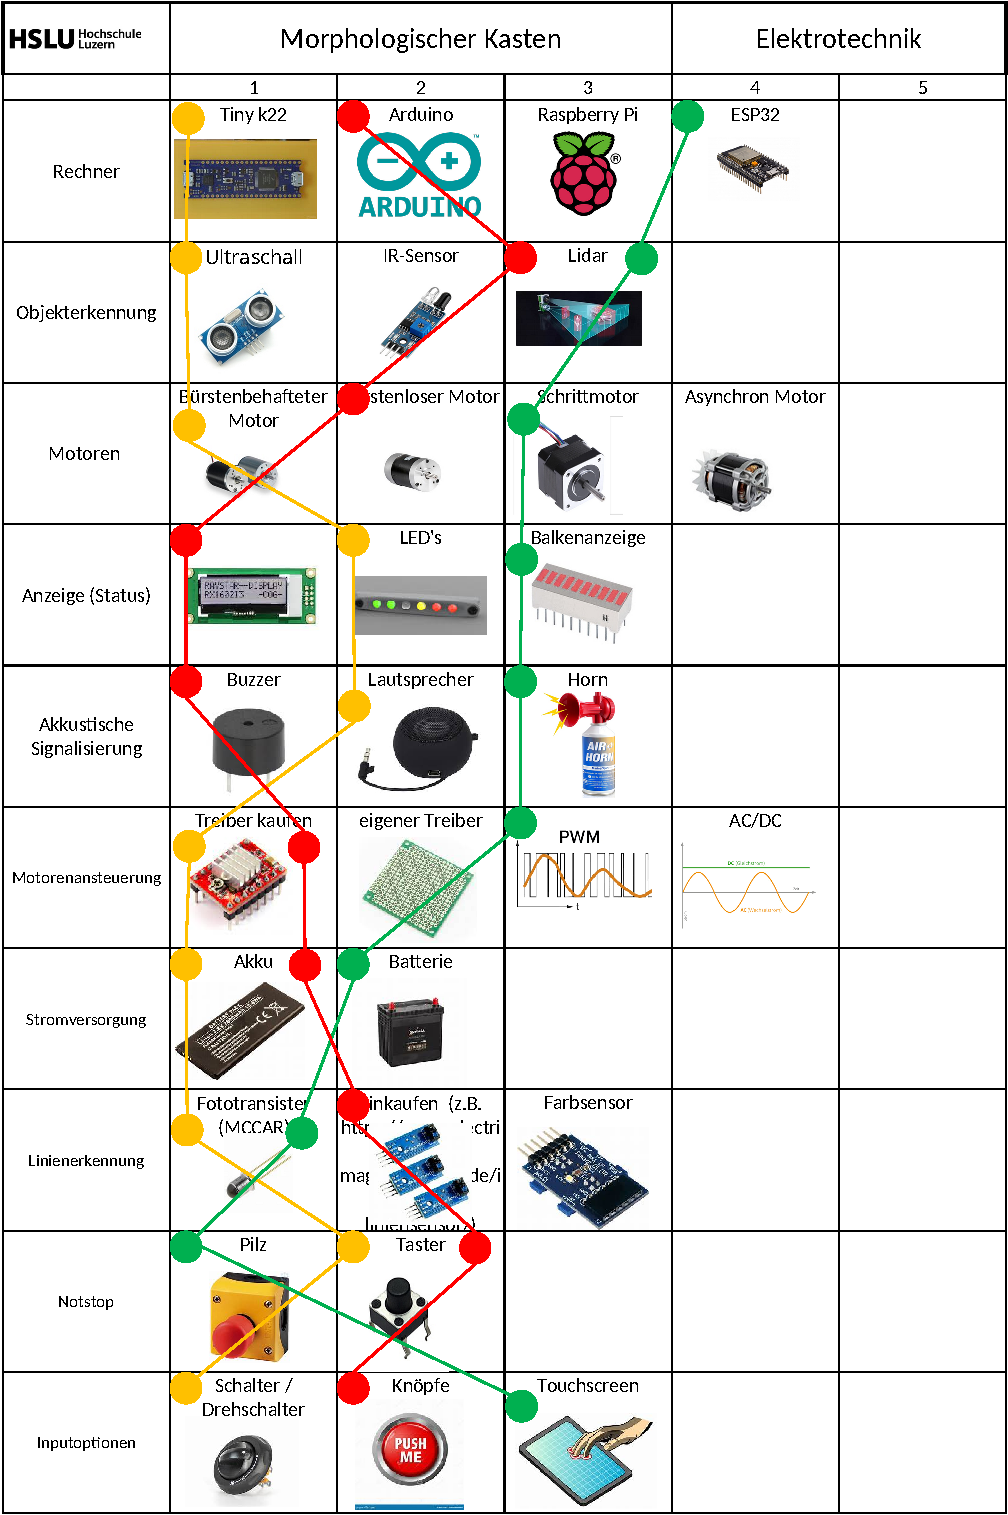
\includegraphics[width=\textwidth -5mm]{assets/MK_Elektrotechnik.pdf}
\caption{Morphologischer Kasten: Steuerung}
\label{table:mk-elektrotechnik}
\end{table}

In allen drei Varianten ist konsequent ein Mikrocontroller vorgesehen. Einige Komponenten, wie etwa Buzzer und Lautsprecher oder Drehschalter und Tasten, sind grösstenteils austauschbar. Spezifische Schaltungselemente wie Strombegrenzer und Spannungsregler wurden hingegen nicht im morphologischen Kasten berücksichtigt, da solche Entscheidungen erst während des Layoutprozesses getroffen werden.


\subsubsection*{Navigation Morphologischer Kasten}
\addcontentsline{toc}{subsubsection}{Navigation Morphologischer Kasten}


Folgender morphologischer Kasten in Tabelle \ref{table:mk-informatik} mit drei Varianten wurde für die Navigation erstellt.  Diese Varianten wurden jeweils aufgrund folgender Kriterien erstellt.

\begin{itemize}
    \item Variante Gelb: Flexibel
    \item Variante Rot: Sicher
    \item Variante Grün: Leichtgewichtig
\end{itemize}

\begin{table}[H]
\centering
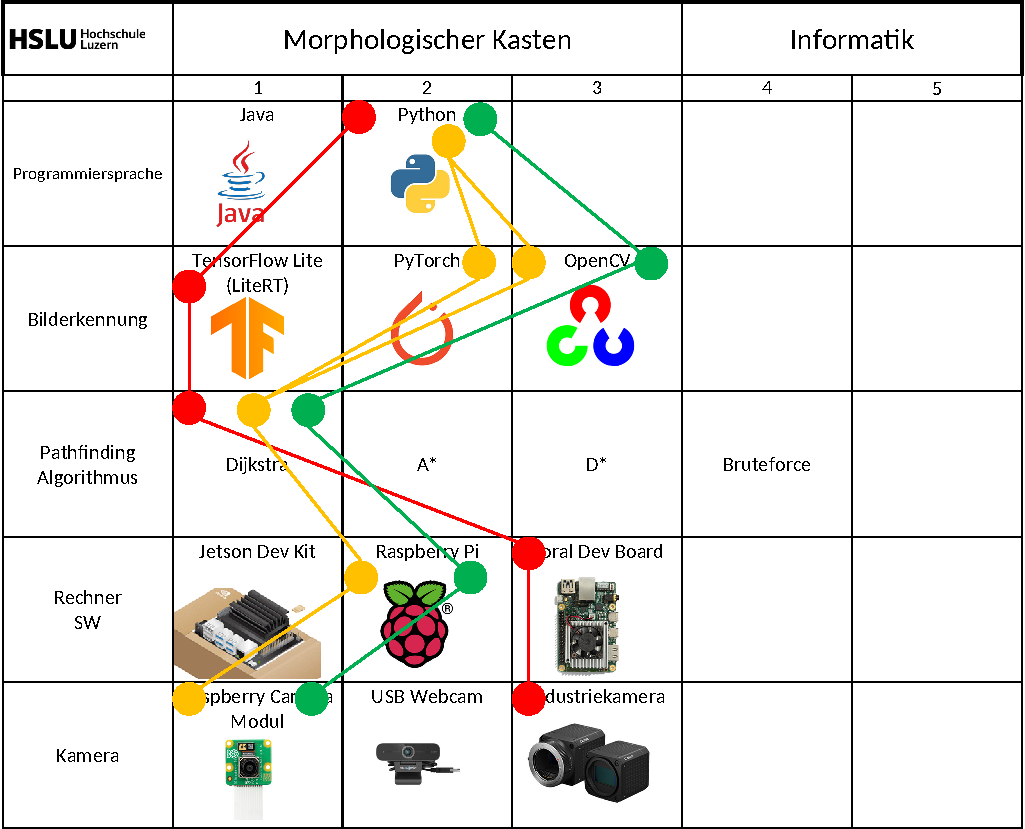
\includegraphics[width=\textwidth]{assets/MK_Informatik.pdf}
\caption{Morphologischer Kasten: Navigation}
\label{table:mk-informatik}
\end{table}


Bei den drei Varianten fällt auf, dass alle Python und den Wegfindealgorithmus \gls{dijkstra} verwenden. Python wurde immer gewählt, da Bilderkennung und Machine Learning sehr gut mit Python harmonisieren. Viele Libraries, inklusive dieser, die hier ersichtlich sind, sind kompatibel mit Python. \gls{dijkstra} wurde immer gewählt, weil dieser Algorithmus simpel und robust ist und die Geschwindigkeit vernachlässigbar ist. Im Graphen gibt es nur 8 Knoten, die Berechnung wird also bei jedem Algorithmus schnell genug sein.

\subsubsection*{Simulator Morphologischer Kasten}\label{mk-simulator}
\addcontentsline{toc}{subsubsection}{Simulator Morphologischer Kasten}



Aus der \nameref{techrecherche} wurde folgender Morphologischer Kasten \ref{table:mk-simulator} für die Teilfunktionen des Simulators erstellt. Es gibt drei Varianten, die in Frage kommen. Diese wurden jeweils nach folgenden Kriterien zusammengestellt.

\begin{itemize}
    \item Variante Gelb: Schnell
    \item Variante Rot: Leichtgewichtig
    \item Variante Grün: Wiederverwendbar im Roboter
\end{itemize}


\begin{table}[H]
\centering
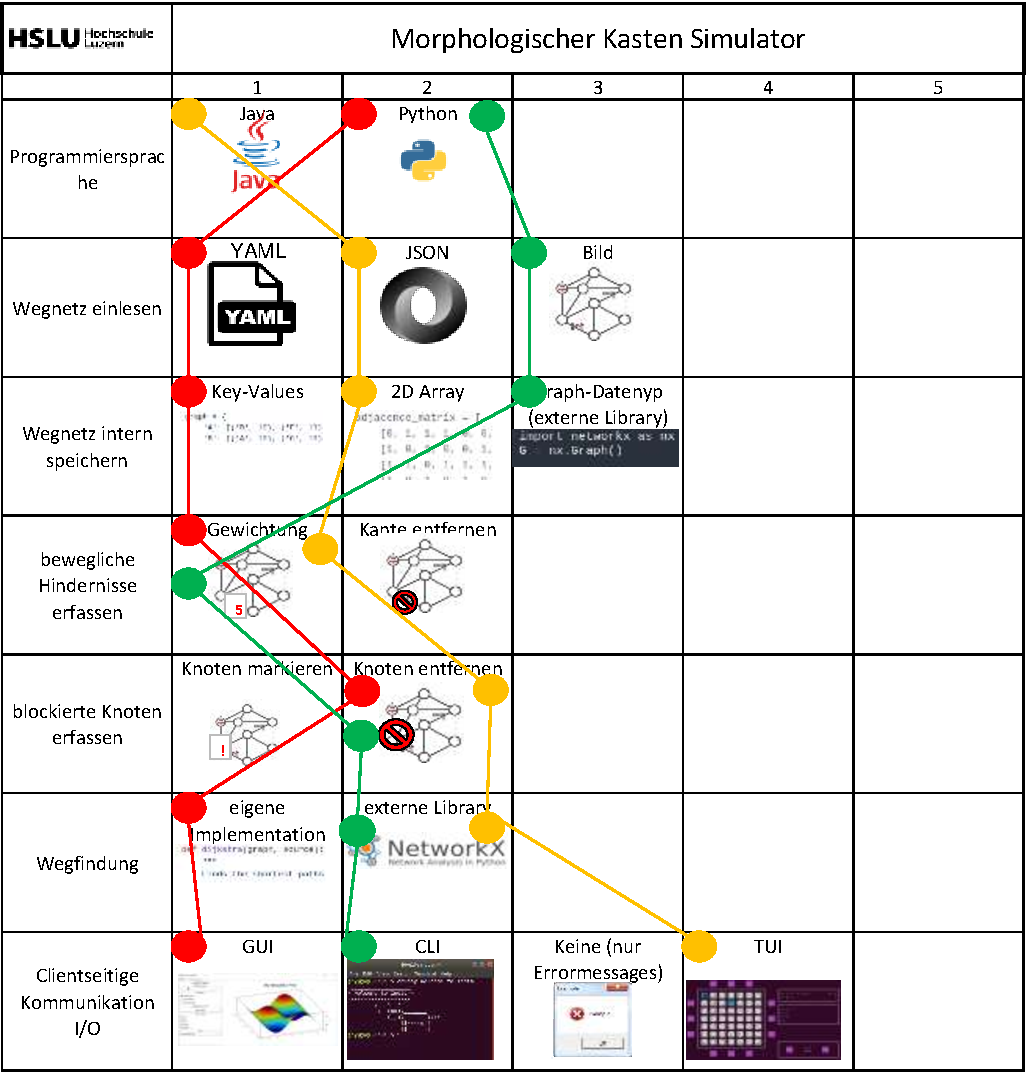
\includegraphics[width=\textwidth]{assets/MK_Simulator.pdf}
\caption{Morphologischer Kasten: Simulator}
\label{table:mk-simulator}
\end{table}



Beim Erfassen von beweglichen Hindernissen, wird in jeder Lösungsvariante die Kante nicht entfernt, sondern neu gewichtet. Es ist nicht garantiert, dass es immer einen Weg ohne beweglichem Hindernisse gibt. Diese Strecken zu entfernen, wäre zu risikobehaftet.

Ebenfalls wird ein Knoten immer entfernt falls, ein Pylon darauf steht. Er wird nicht markiert, da es  keinen Vorteil bringen würde, den Knoten weiterhin zu speichern.


\newpage
\subsection*{Auswahl Lösungskombinationen}\label{nutzwertanalyse}
\addcontentsline{toc}{subsection}{Auswahl Lösungskombinationen}


Zur Auswahl der passendsten Lösungskombination wird pro Teilbereich eine Nutzwertanalyse erstellt. Diese beinhaltet die drei erarbeiteten Varianten aus dem morphologischen Kasten. Die Kriterien und deren Gewichtung sind individuell pro Teilbereich, damit sie ideal passen. Die Variante mit der höchsten Punktzahl ist die Variante, die am besten passt.

\subsubsection*{Mechanik Nutzwertanalyse}
\addcontentsline{toc}{subsubsection}{Mechanik Nutzwertanalyse}

Tabelle \ref{table:nutzwert-maschinentechnik} zeigt die Nutzwertanalyse der drei Lösungskombinationen aus der Mechanik. 

\begin{itemize}
    \item Variante A - Gelb: Zwei von drei Rädern werden direkt durch einen Motor angetrieben. Das dritte Rad ist frei drehend und dient als Stützrad. Das Hindernis wird mit einem Greifer angehoben, der zwei flexible Backen hat, die sich optimal an das Hindernis anpassen. Da Variante A nur drei Räder hat, hat das Chassis die Form eines freien Polygons. Diese Variante zeichnet sich durch ihre effiziente Bauweise aus. 
    \item Variante B - Rot: Die vier Mecanum Räder sind auf der halbrunden Grundplatte angeordnet. Jedes Rad wird mit einem seperaten Motor angetrieben.  Das Hindernis wird mit einer Gabel wie bei einem Gabelstapler angehoben. Diese Variante stellt eine präzise Verschiebung des Hindernisses sicher, ist jedoch in in der Umsetzung aufwändiger als die Variante A. 
    \item Variante C - Grün: Der Antrieb erfolgt mit einem Motor und wird mit mithilfe eines Überlagerungsgetriebes auf die einzelnen Raupen übertragen.  Das Hindernis wird mit einem selbst-klemmenden Seilzuggreifer angehoben. Das Fahrzeug wird auf einem runden Chassis aufgebaut. Aufgrund des Raupenantrieb ist die Variante C die Robusteste der drei Varianten. 
\end{itemize}

\begin{table}[H]
\centering
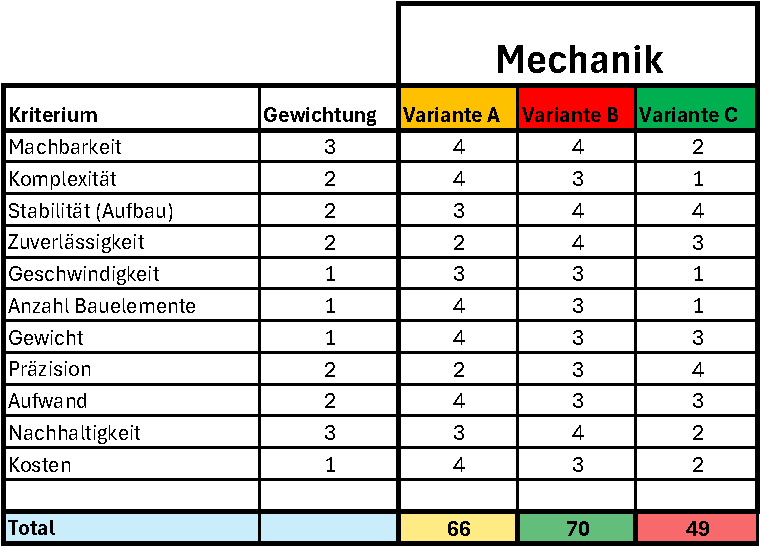
\includegraphics[width=0.75\textwidth]{assets/Nutzwertanalyse-M.pdf}
\caption{Nutzwertanalyse: Mechanik}
\label{table:nutzwert-maschinentechnik}
\end{table}

Die Analyse der drei genannten Varianten hat ergeben, dass die Variante A sich am besten für die Umsetzung eignet. Entsprechend wurden folgende Komponenten und Systeme ausgewählt. 

\begin{itemize}
    \item Fortbewegung: Räder 
    \item Anordnung:  Zwei Räder hinten und ein Stützrad vorne
    \item Lenkung: Direkt Antrieb für zwei Räder
    \item Hebevorrichtung: Greifer Backen mit flexiblen Backen
    \item Chassis: Freies Polygon
\end{itemize}

\subsubsection*{Steuerung Nutzwertanalyse}
\addcontentsline{toc}{subsubsection}{Steuerung Nutzwertanalyse}


Mithilfe des morphologischen Kastens wurden verschiedene Lösungsvarianten aufgezeigt. Die Varianten bestehen aus diversen Komponenten. 
Nun werden drei Varianten in der Nutzwertanalyse in Tabelle \ref{table:nutzwert-ET} evaluiert.

\begin{itemize}
    \item Variante A - Gelb: Das Verwenden vom \gls{tinyk22} macht das System echtzeitfähig. Leichte Motoren werden eingesetzt. Inputs und Outputs werden einfach gehalten über Leuchten und Schalter. Für die Motorsteuerug werden die Treiber eingekauft.
    \item Variante B - Rot: Bei dieser Variante werden die Bauteile Raspberry Pi tauglich verwendet, dies ist also eine ``Plug and Play'' Methode. Ebenfalls haben die Motoren ein geringes Gewicht.
    \item Variante C - Grün: Durch die Schrittmotoren und die Objekterkennung mit \acrfull{lidar}, weist diese Kombination eine hohe Präzision auf. Mit dem Horn als akustisches Signal, wäre das Erreichen des Ziels auffällig. Aufgrund der Schrittmotoren wird der Roboter schwer, was ein Nachteil ist.
\end{itemize}


\begin{table}[H]
\centering
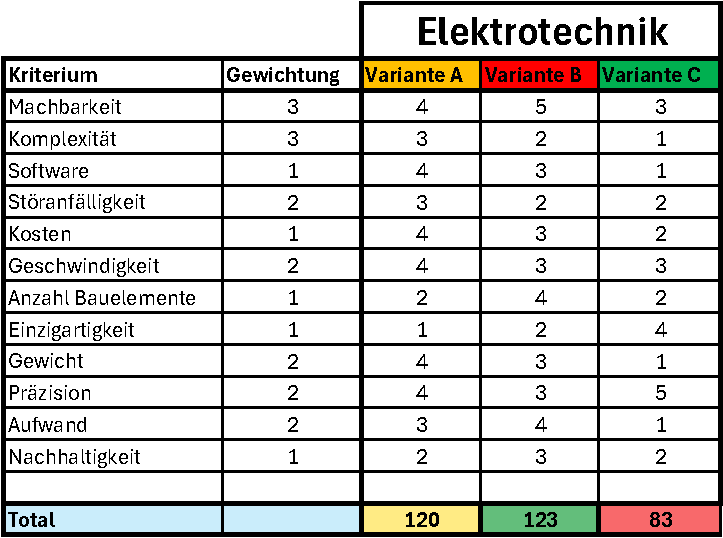
\includegraphics[width=0.75\textwidth]{assets/Nutzwertanalyse-ET.pdf}
\caption{Nutzwertanalyse: Steuerung}
\label{table:nutzwert-ET}
\end{table}

Aus den Bewertungen aus der Nutzwertanalyse zeigt sich die Variante A als höchst bewertete. Somit wird diese Variante weiter verfolgt und besteht aus folgenden Komponenten.

\begin{itemize}
    \item Rechner: \gls{tinyk22}
    \item Objekterkennung: Ultraschall
    \item Motoren: Bürstenbehafteter Motor
    \item Anzeige: \acrshort{led}s
    \item Akkustische Signalisierung: Lautsprecher
    \item Motorenansteuerung: Treiber einkaufen
    \item Stromversorgung: Akku
    \item Linienerkennung: Fototransistor
    \item Not-Stop: Taster
    \item Inputoption: Schalter
\end{itemize}

\subsubsection*{Navigation Nutzwertanalyse}
\addcontentsline{toc}{subsubsection}{Navigation Nutzwertanalyse}

Die drei ermittelten Varianten aus dem vorherigen Kapitel werden analysiert und bewertet mithilfe der Nutzwertanalyse in Tabelle \ref{table:nutzwert-informatik}.

\begin{itemize}
     \item Variante A - Gelb: Python verwendet eine Mischung aus \gls{pytorch} und \gls{opencv}, um \acrshort{ai} und reine Bilderkennung zu verwenden. Durch die verschiedenen Möglichkeiten, ist die Entwicklung sehr flexibel. \gls{dijkstra} berechnet den Weg. Das Ganze rechnet auf einem Raspberry Pi mit einer Raspberry Camera angeschlossen. Diese Methode ist robust, da zwei Möglichkeiten zur Erkennung des Graphens verwendet werden können. Die Kamera und das Board passen gut zusammen und sind recht günstig. 
    \item  Variante B - Rot: Python verwendet LiteRT, um mit AI die Umgebung zu erkennen und \gls{dijkstra}, um den Weg zu berechnen. Das Ganze rechnet auf einem Coral Dev Board und fotografiert den Graphen mit einer Industriekamera. Mit Tensorflow könnten alle Hindernisse sicher erkannt werden, was diese Variante sehr sicher macht. Jedoch ist dies auch ein relativ grosser Algorithmus. Das Coral Dev Board ist stärker als ein Raspberry Pi, aber auch teurer.
    \item Variante C - Grün: Python verwendet nur \gls{opencv} zur Bilderkennung und berechnet mit \gls{dijkstra} den Weg, es rechnet auf einem Raspberry Pi mit einer Raspberry Camera. Diese Variante könnte schwierig werden, da möglicherweise nicht alle Elemente erkannt werden können, wäre aber sehr leichtgewichtig, da keine AI verwendet wird.
\end{itemize}


\begin{table}[H]
\centering
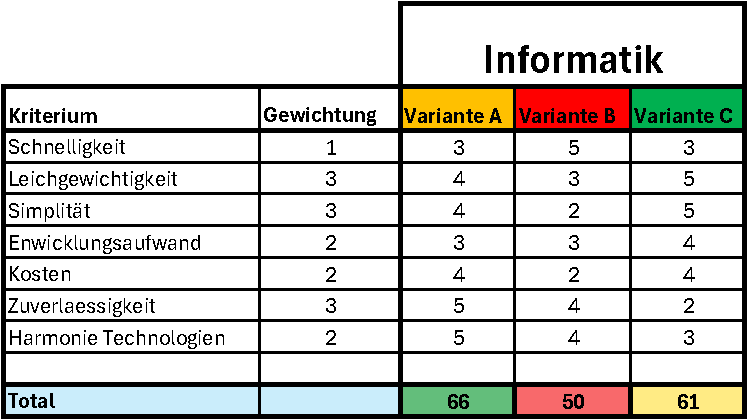
\includegraphics[width=0.75\textwidth]{assets/Nutzwertanalyse-I.pdf}
\caption{Nutzwertanalyse: Navigation}
\label{table:nutzwert-informatik}
\end{table}

Aus der Nutzwertanalyse kann abgelesen werden, dass die Variante A mit Python, \gls{pytorch} und \gls{opencv} am besten passt. Die entsprechenden Komponenten aus dieser Variante sind nachfolgend aufgelistet.

\begin{itemize}
    \item Programmiersprache: Python
    \item Bilderkennung: PyTorch und OpenCV
    \item Pathfinding Algorithmus: Dijkstra
    \item Rechner SW: Raspberry Pi
    \item Kamera: Raspberry Camera Modul
\end{itemize}

\subsubsection*{Simulator Nutzwertanalyse}
\addcontentsline{toc}{subsubsection}{Simulator Nutzwertanalyse}

Tabelle \ref{table:nutzwert-Simulator} zeigt die Nutzwertanalyse des Simulators. Die Kriterien und deren Gewichtung sind dieselben, wie bei der Nutzwertanalyse für die Informatik im Roboter. Das Ziel des Simulators ist es, diesen möglichst realistisch und wiederverwendbar für \acrshort{pren2} umzusetzen.

\begin{itemize}
    \item Variante A: Ein Java Simulator liest ein \gls{json} File mit dem Basegraph und den Hindernissen und speichert es in einem 2D Array. Durch die Verwendung von Java, wäre diese Variante sehr schnell. Bei einem beweglichen Hindernis wird die Gewichtung der Kante erhöht, bei einem Pylonen wird der Knoten entfernt. \gls{dijkstra} wird mit einer externen Library implementiert. Die Aktivitäten des Roboters werden in einem \acrfull{tui} dargestellt. Im richtigen Roboter wird wahrscheinlich nicht Java verwendet werden. Deswegen könnte der Code hier nicht wiederverwendet werden.
    \item Variante B: Ein Python Simulator liest ein \gls{yaml} File mit dem Basegraph und den Hindernissen und speichert es in einem Dictionary. Dies sind alles leichtgewichtige Technologien. Bei einem beweglichen Hindernis wird die Gewichtung der Kante erhöht, bei einem Pylonen wird der Knoten entfernt. \gls{dijkstra} wird selber implementiert, die Aktivitäten des Roboters sind in einem \acrfull{gui} ersichtlich. Der Code kann einfach wiederverwendet werden, unter anderem durch die wenigen externen Abhängigkeiten und die Leichtgewichtigkeit. 
    \item Variante C: Ein Python Simulator liest ein Bild eines Graphens ein und speichert es in einem Graph Datentyp. Bei einem beweglichen Hindernis wird die Gewichtung der Kante erhöht, bei einem Pylonen wird der Knoten entfernt. Eine externe Library implementiert \gls{dijkstra}, die Aktivitäten des Roboters werden in einem \acrfull{cli} dargestellt. Es wird bereits an der Bilderkennung gearbeitet, diese müsste folglich bereits früh definiert sein. Dadurch wären bereits viele Aspekte implementiert, die der Roboter brauchen wird.
\end{itemize}

\begin{table}[H]
\centering
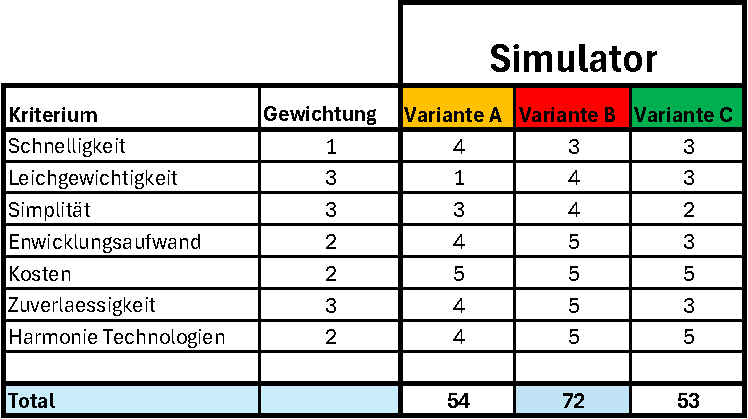
\includegraphics[width=0.75\textwidth]{assets/Nutzwertanalyse-Simulator.pdf}
\caption{Nutzwertanalyse: Simulator}
\label{table:nutzwert-Simulator}
\end{table}

Die Nutzwertanalyse zeigt, dass die Variante B: Python mit \gls{yaml} und einem \acrshort{gui} am besten abschneidet. Diese Variante besteht aus folgenden Teilen.

\begin{itemize}
    \item Programmiersprache: Python
    \item Wegnetz einlesen: \gls{yaml}
    \item Wegnetz intern speichern: Key-Values
    \item Bewegliche Hindernisse erfassen: Gewichtung
    \item Blockierte Knoten erfassen: Knoten entfernen
    \item Wegfindung: eigene Implementation
    \item Clientseitige Kommunikation \acrshort{i/o}: \acrshort{gui}
\end{itemize}